\documentclass[journal]{IEEEtran}
\usepackage{amsmath,amssymb,bm,booktabs,array,tabularx,multirow,graphicx,cite,url,xcolor,balance}
\usepackage{xurl}
\usepackage{tikz}
\usetikzlibrary{arrows.meta,positioning,calc}
\definecolor{rfInk}{HTML}{23272A}
\definecolor{rfRule}{HTML}{818A8F}
\definecolor{rfAccent}{HTML}{245769}
\usepackage[hidelinks]{hyperref}
\hypersetup{pdftitle={Hierarchical RF Tokenization for Parameter-Efficient Cross-Receiver LoRa Fingerprint Identification},pdfauthor={Anonymous working draft},pdfsubject={Parameter-efficient radio-frequency fingerprint identification},pdfkeywords={LoRa, RF fingerprinting, hierarchical tokenization}}
\graphicspath{{figures/}}
\setlength{\tabcolsep}{4pt}
\begin{document}
\title{Hierarchical RF Tokenization for Parameter-Efficient Cross-Receiver LoRa Fingerprint Identification}
\author{Anonymous working draft}
\markboth{Hierarchical RF Tokenization for Cross-Receiver LoRa Identification}{Hierarchical RF Tokenization for Cross-Receiver LoRa Identification}
\maketitle
\begin{abstract}
The tokenizer determines how local radio-frequency (RF) features are compressed before global attention. We study how this step affects cross-receiver fingerprint identification and develop HStem, a four-stage convolutional tokenizer that progressively combines local features. In a LoRa comparison with matched input views, token geometry, nominal convolutional support, and attention architecture, HStem improves accuracy over a direct Long-Patch projection by 2.835 percentage points and leads in all six paired fits. In the Native baseline comparison with five training receivers per fold and 160 training packets per transmitter--receiver pair, HStem achieves 97.333\% receiver-equal accuracy and 93.683\% worst-receiver accuracy with 133,690 parameters. The strongest external comparator, a Spec+Siamese reimplementation, reaches 95.890\% under the same packet and receiver protocol. HStem uses 0.96\% of its parameters and delivers 1.96 times its batch-128 throughput in a shared GPU session. A matched WiFi stress test also shows smaller accuracy losses under controlled frequency and timing perturbations.
\end{abstract}
\begin{IEEEkeywords}
Radio-frequency fingerprint identification, LoRa, cross-receiver identification, tokenization, parameter efficiency, representation analysis.
\end{IEEEkeywords}


\section{Introduction}
\IEEEPARstart{R}{adio-frequency} fingerprint identification (RFFI) uses hardware-dependent waveform signatures to distinguish enrolled transmitters. A classifier trained with one set of receivers must recover those signatures from observations distorted by different receiver chains and propagation conditions \cite{zhang2025survey}. For an attention-based classifier, the tokenizer determines which combinations of local RF features reach the attention blocks. This makes token formation a practical design choice for both identification accuracy and inference cost.

Prior LoRa methods address receiver variation through channel-independent signal representations, receiver-adversarial training, and cross-receiver contrastive learning \cite{shen2022scalable,shen2024receiver,ma2025robust}. We study the intervening step that converts the output of the RF front-end, an \(8192\times32\) feature array, into a \(32\times64\) token sequence. How much can token construction change identification accuracy when the input representation, nominal local support, output geometry, and attention architecture are matched? A direct long projection aggregates a token's neighborhood in one spatial step. Progressive tokenization transforms features at intermediate resolutions before the final compression.

HStem realizes progressive tokenization with four strided local convolutional stages (Fig.~\ref{fig:architecture}). The first three combine overlapping neighborhoods, with batch normalization (BN) and a Gaussian error linear unit (GELU) at each resolution. The last forms the sequence for two standard multihead attention (MHA) blocks. We construct a freely learned Long-Patch projection with matched nominal span, stride, and first-token center and 3.48\% more model parameters. The paired models train end to end with transmitter cross-entropy and matched initial states for the shared front-end and backend.

\begin{figure*}[t]\centering
% The IQ traces and feature maps are schematic.
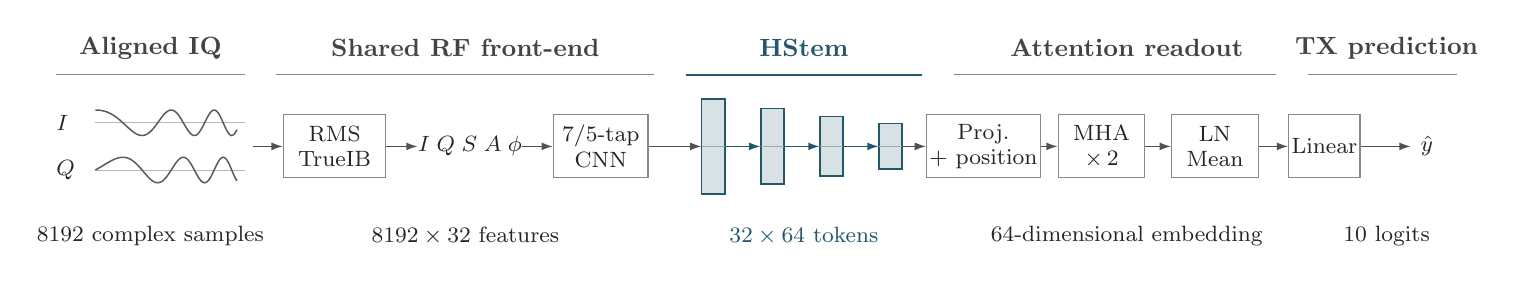
\begin{tikzpicture}[
  x=1mm,y=1mm,font=\fontsize{8}{9.2}\selectfont,text=rfInk,
  heading/.style={font=\fontsize{8.6}{10}\selectfont\bfseries,text=rfInk!86},
  measure/.style={font=\fontsize{7.7}{9}\selectfont},
  operator/.style={draw=rfRule,fill=white,line width=.42pt,
    minimum height=8mm,inner sep=1pt,align=center},
  flow/.style={-{Latex[length=1.45mm,width=1mm]},draw=rfInk!80,line width=.54pt}]

\node[heading] at (12,29) {Aligned IQ};
\node[heading] at (52,29) {Shared RF front-end};
\node[heading,font=\fontsize{9}{10}\selectfont\bfseries,text=rfAccent] at (95,29) {HStem};
\node[heading] at (136,29) {Attention readout};
\node[heading] at (169,29) {TX prediction};
\foreach \leftedge/\rightedge in {0/24,28/76,114/155,159/178}
  \draw[rfRule,line width=.42pt] (\leftedge,25.6) -- (\rightedge,25.6);
\draw[rfAccent,line width=.85pt] (80,25.6) -- (110,25.6);

% Analytic quadrature pair for the input window.
\foreach \height/\component/\phase in {19.5/I/0,13.5/Q/-90} {
  \node[measure,anchor=west,inner sep=0pt] at (0,\height) {$\component$};
  \draw[rfRule!60,line width=.35pt] (5,\height) -- (24,\height);
  \draw[rfInk!76,line width=.54pt,samples=105,domain=0:18,variable=\u]
    plot ({5+\u},{\height+1.62*cos(19*\u+1.9*\u*\u+\phase)});
}

\node[operator,minimum width=13mm] (band) at (35.4,16.5) {RMS\\TrueIB};
\node[measure,inner sep=0pt] (views) at (52.6,16.5) {$I\;Q\;S\;A\;\phi$};
\node[operator,minimum width=12mm] (cnn) at (69.2,16.5) {7/5-tap\\CNN};
\draw[flow] (25,16.5) -- (band.west);
\draw[flow] (band.east) -- (views.west);
\draw[flow] (views.east) -- (cnn.west);
\draw[flow] (cnn.east) -- (82,16.5);

% Four feature maps at progressively shorter sequence lengths.
\foreach \center/\halfheight in {83.5/6.0,91/4.8,98.5/3.8,106/2.9} {
  \draw[rfAccent,fill=rfAccent!18,line width=.63pt]
    (\center-1.5,16.5-\halfheight) rectangle (\center+1.5,16.5+\halfheight);
  \draw[rfAccent!50,line width=.32pt]
    (\center-1.5,16.5) -- (\center+1.5,16.5);
}
\foreach \leftedge/\rightedge in {85/89.5,92.5/97,100/104.5}
  \draw[flow,draw=rfAccent,line width=.63pt] (\leftedge,16.5) -- (\rightedge,16.5);

\node[operator,minimum width=12mm] (position) at (117.8,16.5) {Proj.\\$+$ position};
\node[operator,minimum width=11mm] (attn) at (132.8,16.5) {MHA\\$\times\,2$};
\node[operator,minimum width=11mm] (pool) at (147.2,16.5) {LN\\Mean};
\node[operator,minimum width=9mm] (linear) at (161.1,16.5) {Linear};
\node (prediction) at (174.1,16.5) {$\hat y$};
\draw[flow] (107.5,16.5) -- (position.west);
\draw[flow] (position.east) -- (attn.west);
\draw[flow] (attn.east) -- (pool.west);
\draw[flow] (pool.east) -- (linear.west);
\draw[flow] (linear.east) -- (prediction.west);

\node[measure] at (12,5.1) {$8192$ complex samples};
\node[measure] at (52,5.1) {$8192 \times 32$ features};
\node[measure,text=rfAccent] at (95,5.1) {$32 \times 64$ tokens};
\node[measure] at (136,5.1) {$64$-dimensional embedding};
\node[measure] at (169,5.1) {$10$ logits};
\end{tikzpicture}

\caption{Closed-set LoRa transmitter identification with HStem. TrueIB reconstructs the in-band signal used to form the five views. \(S\), \(A\), and \(\phi\) denote the standardized log-magnitude, log-amplitude, and scaled phase views. The IQ traces and feature maps are schematic.}
\label{fig:architecture}
\end{figure*}

\begin{enumerate}
\item We introduce HStem, which combines overlapping local RF neighborhoods at successive resolutions to form 32 tokens for global attention.
\item We measure the effect of replacing the tokenizer at matched nominal support and interface. HStem gains 2.835\,pp over Long-Patch, with a conditional 95\% receiver interval of \([2.253,3.530]\) pp. Kernel parameterization, the BN--GELU interaction, and layerwise geometry provide complementary evidence about the sources of the gain.
\item On a common LoRa packet and receiver split, HStem reaches 97.333\% accuracy and 97.325\% macro-F1 with 133,690 parameters. It reduces the parameter count by 99.04\% relative to Spec+Siamese and delivers 1.96 times its batch-128 throughput in the shared GPU session.
\end{enumerate}

\section{Related Work}
Channel-independent signal representations provide an important LoRa baseline \cite{shen2022scalable}. Shen et al.\ combine CIS with receiver-adversarial learning \cite{shen2024receiver}, adapting gradient-reversal domain training \cite{ganin2016domain} to receiver hardware. Our CE and DANN comparisons retain the same encoder and transmitter head and vary the use of source-RX supervision.

Ma et al.\ use spectrograms and contrastive training on same-transmitter pairs from different receivers \cite{chen2020simclr,ma2025wcnc,ma2025robust}. Triad-GAN augments the embedding learner with a transmitter-conditioned generator and discriminator \cite{wang2026triad}. RIFLE combines a residual encoder with receiver-adversarial training for deployments with partial transmitter--receiver coverage \cite{zhang2026rifle}. Table~\ref{tab:protocol-context} summarizes these studies' evaluation contexts.

FAN/IB-RFF and ASKNet use frequency-aware features, information bottlenecks, and spectral dynamics \cite{wang2026ib,liu2026ask}. Federated contrastive learning, feature alignment, and domain-adversarial aggregation address distributed receiver data \cite{shen2024federated,wang2026fedalign,gul2026federated}.

CvT combines convolutional token embeddings with convolutional attention projections, PVT forms a spatial pyramid, and Swin links shifted attention windows \cite{wu2021cvt,wang2021pvt,liu2021swin}. RF Transformer work addresses variable-length LoRa inputs \cite{shen2023length}, GFSK classification \cite{herrera2026transformer}, and segmented or multiscale WiFi features \cite{hui2025cross,yang2026sinformer}. Our RF study varies the tokenizer before two standard MHA blocks and evaluates it against a projection with the same local convolution-path support. The design uses established attention and normalization operators \cite{vaswani2017attention,ioffe2015batch,ba2016layer}. Shift-stability work \cite{zhang2019shift} motivates our alignment stress tests.

\section{Signal Model and Identification Task}
Let $y\in\{1,\ldots,10\}$ identify an enrolled physical transmitter and $r$ denote the receiver. We model a received window as
\begin{equation}
 x=\mathcal{R}_{r}\!\left(\mathcal{C}_{\eta}
       \left(\mathcal{T}_{y}(s)\right)\right)+n ,
\end{equation}
where $\mathcal{T}_{y}$, $\mathcal{C}_{\eta}$, and $\mathcal{R}_{r}$ describe the transmitter, channel, and receiver, respectively, and $n$ denotes noise. We train $f_\theta(x)$ on labeled recordings from source receivers and apply the resulting classifier directly to the same enrolled transmitter identities at held receivers. HStem uses transmitter supervision.

The companion study diagnoses out-of-band dependence with frozen pathway interventions \cite{oobcompanion}. HStem inherits its TrueIB reconstruction, five views, local front-end, and $32\times64$ token interface. We train paired architectures within that common in-band path to measure the effect of token construction.


\section{Hierarchical RF Token Formation}
\subsection{Signal Preprocessing and Five Views}
For $N=8192$, RMS normalization and the discrete in-band projection are
\begin{align}
 \tilde{x}[n]&=x[n]/\sqrt{N^{-1}\sum_m|x[m]|^2+\epsilon},\\
 x_{\mathrm{IB}}&=\mathcal{F}^{-1}
      \left(M\odot\mathcal{F}(\tilde{x})\right),\quad
 M[k]=\mathbf{1}\{|f_k|\leq 62.5\ {\rm kHz}\}.
\end{align}
The mask retains 1025 bins, including DC and the edge bins. Views are I, Q, standardized $\log(1+|\mathrm{FFT}|)$, $\log(1+\sqrt{I^2+Q^2+\epsilon})$, and $\operatorname{atan2}(Q,I)/\pi$. FFT magnitude is fftshift ordered and standardized per window using sample standard deviation, clamped below by $\epsilon=10^{-6}$. The same epsilon is used by RMS and amplitude construction. These inherited definitions are fixed for every tokenizer control.

The inherited representation concatenates frequency-indexed FFT magnitudes with sample-indexed I/Q, amplitude, and phase at the same numerical indices. We measure support in this feature coordinate system. TrueIB and the FFT view depend on the full acquired window.

\subsection{Shared Front-End and Tokenizer}
The shared front-end has stride-one kernel-7 and kernel-5 convolutions, each with 32 channels, BN, and LeakyReLU. HStem maps the resulting \(8192\times32\) feature array to \(32\times64\) tokens with four strided convolutions (Table~\ref{tab:arch}). BN and GELU follow the first three stages, and the last stage is an affine convolution.

Figure~\ref{fig:architecture} follows the signal from aligned IQ to transmitter prediction. The backend adds learned position terms after input projection and applies pre-normalization followed by two four-head MHA blocks. Each block uses scaled dot-product attention, output projection, and a normalized residual. Final layer normalization and mean pooling give a 64-dimensional embedding for the linear TX head. The full model has 133,690 parameters.

\subsection{Matched and Mechanism Controls}
Long-Patch uses a grouped kernel-340/stride-256 projection from 32 to 64 channels (eight groups, padding 42), followed by pointwise 64-to-64 mixing. It matches HStem's output geometry and nominal support at 138,346 parameters (Fig.~\ref{fig:matched-tokenizers}). Patch-Lite (P0) uses kernel 256 and width 80 at the same stride and group count, followed by pointwise 80-to-64 mixing. It provides a closer parameter match at 134,266 parameters and a shorter support.

\begin{figure*}[t]\centering
% Spatial dimensions are reported as positions x channels.
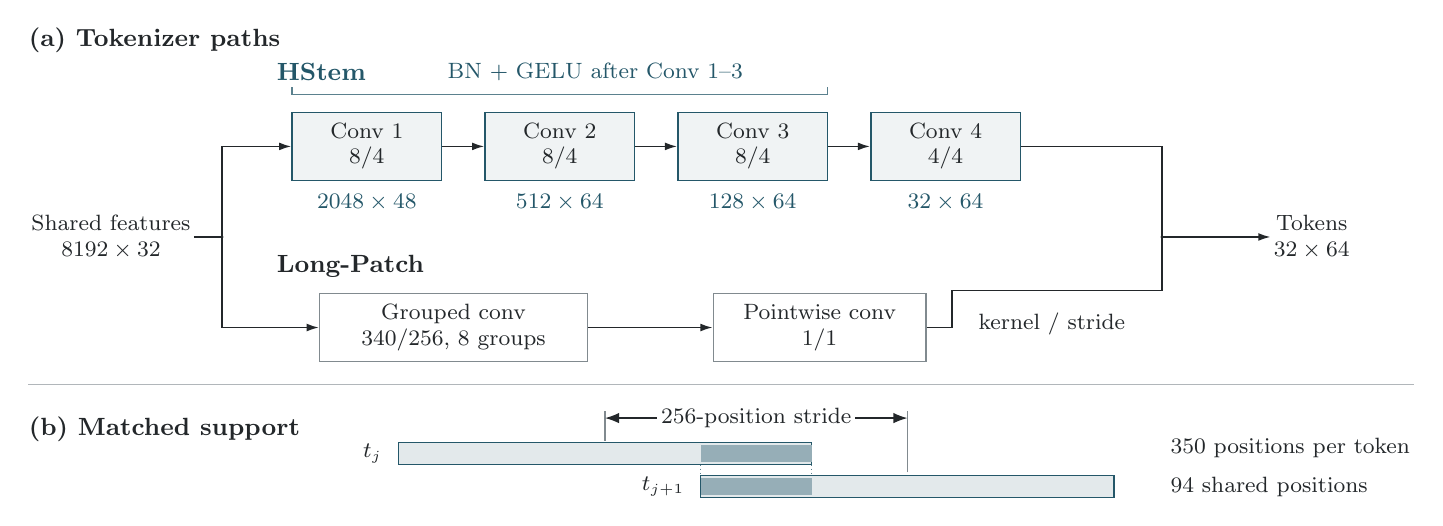
\begin{tikzpicture}[
  x=1mm,y=1mm,font=\fontsize{8}{9.2}\selectfont,text=rfInk,
  title/.style={font=\fontsize{8.6}{10}\selectfont\bfseries,anchor=west,inner sep=0pt},
  size/.style={font=\fontsize{7.7}{9}\selectfont,inner sep=0pt},
  operation/.style={draw=rfRule,fill=white,line width=.52pt,
    minimum height=8.6mm,minimum width=19mm,align=center,inner sep=1pt},
  stage/.style={operation,draw=rfAccent,fill=rfAccent!7},
  flow/.style={-{Latex[length=1.55mm,width=1mm]},draw=rfInk,line width=.6pt}]

\node[title] at (0,59) {(a) Tokenizer paths};
\node[title,text=rfAccent] at (31.5,55) {HStem};
\node[size,text=rfAccent] at (72,55) {BN + GELU after Conv 1--3};
\draw[rfAccent!75,line width=.45pt] (33.5,53)
  -- (33.5,52.1) -- (101.5,52.1) -- (101.5,53);
\node[stage] (conv1) at (43,45.5) {Conv 1\\$8/4$};
\node[stage] (conv2) at (67.5,45.5) {Conv 2\\$8/4$};
\node[stage] (conv3) at (92,45.5) {Conv 3\\$8/4$};
\node[stage] (conv4) at (116.5,45.5) {Conv 4\\$4/4$};
\node[size,text=rfAccent] at (43,38.4) {$2048 \times 48$};
\node[size,text=rfAccent] at (67.5,38.4) {$512 \times 64$};
\node[size,text=rfAccent] at (92,38.4) {$128 \times 64$};
\node[size,text=rfAccent] at (116.5,38.4) {$32 \times 64$};

\node[title] at (31.5,30.3) {Long-Patch};
\node[operation,minimum width=34mm] (grouped) at (54,22.5) {Grouped conv\\$340/256$, 8 groups};
\node[operation,minimum width=27mm] (pointwise) at (100.5,22.5) {Pointwise conv\\$1/1$};
\node[size] at (130,23) {kernel / stride};

\node[align=center,inner sep=1pt] (features) at (10.5,34)
  {Shared features\\$8192 \times 32$};
\node[align=center,inner sep=1pt] (tokens) at (163,34)
  {Tokens\\$32 \times 64$};
\draw[rfInk,line width=.6pt] (features.east) -- (24.6,34);
\draw[flow] (24.6,34) |- (conv1.west);
\draw[flow] (24.6,34) |- (grouped.west);
\draw[flow] (conv1) -- (conv2);
\draw[flow] (conv2) -- (conv3);
\draw[flow] (conv3) -- (conv4);
\draw[flow] (grouped) -- (pointwise);
\draw[rfInk,line width=.6pt] (conv4.east) -| (144,34);
\draw[rfInk,line width=.6pt] (pointwise.east) -- (117.3,22.5)
  -- (117.3,27.2) -| (144,34);
\draw[flow] (144,34) -- (tokens.west);
\fill[rfInk] (24.6,34) circle[radius=.62pt];
\fill[rfInk] (144,34) circle[radius=.62pt];

% Two adjacent interior windows at .15 mm per coordinate position.
\draw[rfRule!62,line width=.44pt] (0,15.3) -- (176,15.3);
\node[title] at (0,9.6) {(b) Matched support};
\node[size,anchor=east] at (45,6.5) {$t_j$};
\node[size,anchor=east] at (83.4,2.3) {$t_{j+1}$};
\draw[rfAccent,fill=rfAccent!13,line width=.46pt] (47,5.1) rectangle (99.5,7.9);
\draw[rfAccent,fill=rfAccent!13,line width=.46pt] (85.4,.9) rectangle (137.9,3.7);
\fill[rfAccent!48] (85.4,5.4) rectangle (99.5,7.6);
\fill[rfAccent!48] (85.4,1.2) rectangle (99.5,3.4);
\draw[rfAccent!75,densely dotted,line width=.5pt] (85.4,5.1) -- (85.4,3.7)
  (99.5,5.1) -- (99.5,3.7);
\draw[rfRule,line width=.46pt] (73.25,8.1) -- (73.25,11.9)
  (111.65,4.1) -- (111.65,11.9);
\draw[Latex-Latex,rfInk,line width=.46pt] (73.25,11) -- (111.65,11);
\node[size,fill=white,inner xsep=1.3pt] at (92.45,11) {$256$-position stride};
\node[size,anchor=west] at (145,7.2) {$350$ positions per token};
\node[size,anchor=west] at (145,2.3) {$94$ shared positions};
\end{tikzpicture}

\caption{Token construction at matched support. (a) HStem builds tokens progressively, and Long-Patch uses a grouped long projection with pointwise channel mixing. Labels inside the blocks give kernel width and stride. The paths use the same front-end and attention architectures. Parameter counts describe the full models, and accuracies are receiver-equal means from the matched GPU evaluation across two folds and three seeds. (b) With the front-end included, both paths span 350 feature positions per interior token and share 94 positions between adjacent tokens.}
\label{fig:matched-tokenizers}
\end{figure*}

H1 expands the learned P0 kernel from 256 to 340 taps by fixed scaled interpolation, retaining stride 256 and padding 42. S1 applies a full-rank 256-to-340-to-256 round trip while retaining the original output support. H2 removes three intermediate tokenizer BN modules; S2 substitutes channel-wise affine transformations, retaining their 352 affine parameters without their statistics.

Including the shared front-end, P0/S1 have local feature-coordinate support 266 and H0/H1/H2/S2 support 350. All have stride 256 and first-token center 127.5. The S1--P0 and H1--S1 contrasts test changes to parameterization at fixed support and then to the expanded-kernel configuration. H2 and S2 test the contribution of train-time normalization.


\subsection{Support Growth and Coordinate Compression}
Let $N_l,C_l$ denote length and channels after stage $l$, and $J_l,R_l,c_l$ denote its jump, nominal convolution-path support, and first-center coordinate. With kernel $k_l$, stride $s_l$, dilation one, and padding $p_l$,
\begin{align}
N_l&=\left\lfloor\frac{N_{l-1}+2p_l-k_l}{s_l}\right\rfloor+1,\\
J_l&=s_lJ_{l-1},\quad R_l=R_{l-1}+(k_l-1)J_{l-1},\\
c_l&=c_{l-1}+\left((k_l-1)/2-p_l\right)J_{l-1}.
\end{align}
The common front-end gives $R_0=11,J_0=1,c_0=0$. HStem consequently has supports $18,46,158,350$, lengths $2048,512,128,32$, and final center 127.5. Its tokenizer alone spans 340 front-end positions. Including the shared front-end, P0 and Long-Patch have supports 266 and 350 at the same jump of 256.

\begin{table*}[t]\centering
\caption{Progressive coordinate reduction in HStem. $R$ gives the nominal support through the convolutions with BN frozen.}
\label{tab:compression}\label{tab:arch}
\begin{tabular}{lrrrrrrr}\toprule
Position & Kernel & Stride & Pad & Channels & Length & $R$ & Coordinates\\\midrule
Shared input &--&--&--&32&8192&11&262144\\
Stage 1&8&4&2&48&2048&18&98304\\
Stage 2&8&4&2&64&512&46&32768\\
Stage 3&8&4&2&64&128&158&8192\\
Stage 4&4&4&0&64&32&350&2048\\\bottomrule
\end{tabular}\end{table*}

The token interface reduces the coordinate count by a factor of 128, from 262,144 after the shared CNN to 2,048. The first three stages mix overlapping neighborhoods as they downsample, and the last groups four adjacent stage-3 positions. Adjacent output tokens consequently share 94 positions of nominal support (\(350-256\)) in the upstream feature coordinates. Frozen BN is pointwise for this calculation.

\subsection{Long Projection, Nonlinearity, and Budget}
Treat the front-end feature array \(h\) and token array \(z\) as vectors in the following equations. The grouped and pointwise convolutions of Long-Patch compose into an affine map,
\begin{equation}
 z_{\rm LP}=W_{\rm LP}h+b_{\rm LP},\qquad J_{\rm LP}=W_{\rm LP}.
\end{equation}
Let \(K_l\) denote the linear part of HStem's stage-\(l\) convolution and \(b_l\) its bias. Beginning with \(h_0=h\), the first three stages compute
\begin{equation}
 \begin{aligned}
 a_l&=\mathrm{BN}_l(K_lh_{l-1}+b_l),\\
 h_l&=\mathrm{GELU}(a_l),\qquad l=1,2,3 .
 \end{aligned}
\end{equation}
The final convolution gives \(z_H=K_4h_3+b_4\). With frozen BN, the tokenizer Jacobian is
\begin{equation}
 J_H(h)=K_4D_3(h)B_3K_3D_2(h)B_2K_2D_1(h)B_1K_1 ,
\end{equation}
where \(B_l\) holds the frozen BN scales and \(D_l(h)=\mathrm{diag}(\mathrm{GELU}'(a_l))\). The stage derivatives depend on \(h\), so HStem can adapt the local feature transformation to the input before producing each token. This analysis describes the tokenizer mapping. Both complete classifiers include nonlinear front-ends and backends.

A grouped long projection with intermediate width $m$ and $g$ groups has
\begin{equation}
 P_{\rm patch}=P_{\rm shared}+32mk/g+m+64m+64,
\end{equation}
with $P_{\rm shared}=47,082$. P0 uses $m=80,g=8,k=256$. Long-Patch uses $m=64,g=8,k=340$, yielding 138,346 parameters, 3.48\% above HStem. The pointwise layer combines groups so that the long projection can attain output rank 64.

Convolution MACs are \(\sum_lN_lk_lC_{l-1}C_l/g_l\). The shared front-end costs 51.118M convolution MACs. HStem spends 42.467M tokenizer convolution MACs compared with 2.916M for Long-Patch because it operates over more intermediate positions. Its small local kernels keep the parameter count close to Long-Patch's. End-to-end latency and throughput are measured separately.

\section{Dataset and Evaluation Protocol}
\subsection{Shen LoRa Splits}
The public Shen corpus provides 8192-sample complex LoRa windows at 1 MHz, with SF7 and 125 kHz bandwidth \cite{shen2024receiver}. The ten enrolled physical TXs correspond to labels 31--40. P-H5$\times$160 fixes 200 packets per TX/RX, with 160 for source training and 40 for source validation. Each fit uses 8,000 training packets, 2,000 source-validation packets, and 10,000 evaluation packets across five held receivers.

Fold 0 trains on B210-1, RTL-1, RTL-3, RTL-6, and RTL-9 and evaluates on B200-mini-1, Pluto-1, RTL-2, RTL-5, and RTL-7. Fold 1 reverses the roles. Seeds 201/202/203 provide six fits per complete method/view over ten distinct RXs. All ten have prior development history. The six blind RXs evaluated in the companion study remain outside the current experiment.

HStem and its controls train for 200 epochs using cross-entropy, batch size 64, and AdamW \cite{loshchilov2019adamw} with learning rate $10^{-3}$ and weight decay $5\times10^{-4}$. Five warmup epochs precede cosine decay. Source training adds AWGN at nominal SNRs from 0 to 50 dB. Shared initial parameters, permutations, and noise streams pair the architecture fits, with selection by minimum clean source RX-equal TX cross-entropy.


\subsection{Native and Strict-IB Comparisons}
The \emph{Native} comparison gives each method the same raw IQ packets and keeps its own feature pipeline, including HStem's TrueIB. The \emph{Strict-IB} comparison applies the common in-band restriction before the other methods' front-ends. Both views share packet identities, receiver roles, and enrolled transmitters. HStem therefore supplies the same in-band reference in both views.

Shen-CE and Shen-DANN use the same CIS residual encoder with and without adversarial source-RX supervision. The Native comparison includes a paper-derived, from-scratch Spec+Siamese implementation with cross-RX same-TX pairs, channel and noise augmentation, and a classification and NT-Xent objective \cite{ma2025robust}. These comparisons evaluate all models on the common P-H5$\times$160 packet budget. The supplement documents the FAN, IB-RFF, ASKNet, and Gul Federated adaptations and audits their correspondence to the authors' original protocols.

\subsection{Metrics and Paired Estimates}
We average accuracy and macro-F1 with equal receiver weights across the three seeds per RX. Worst-RX accuracy is the minimum of the ten RX means. Fit standard deviations summarize the six fold--seed means. Paired contrasts first average seed differences on each receiver, then use 10,000 paired bootstrap draws over the ten distinct RXs. The intervals describe receiver variation conditional on this fitted cohort and exclude variation across acquisitions and newly trained seeds. Table captions identify the evaluation sessions.


\section{Identification Accuracy and Efficiency}
\subsection{LoRa Baseline Comparisons}
HStem has the highest observed Native accuracy (97.333\%) and macro-F1 (97.325\%) in Table~\ref{tab:external}, using transmitter cross-entropy. Spec+Siamese reaches 95.890\%, followed by Shen-DANN at 94.208\% and Shen-CE at 93.535\%. The observed HStem--Spec+Siamese gap is 1.443\,pp (conditional 95\% interval \([-0.565,3.353]\) pp). With the common in-band restriction, the closest comparator is Shen-CE, with a 2.632\,pp gap to HStem. Table~\ref{tab:paired} reports the paired receiver estimates.

\begin{table*}[t]\centering
\caption{Primary LoRa comparisons on P-H5$\times$160. Accuracy and macro-F1 are RX-equal percentages. Fit SD is over six fold--seed means. Worst RX is the lowest per-receiver seed mean. All models share the evaluation packets. Spec+Siamese is evaluated in Native.}
\label{tab:external}% Generated from the submission evidence ledger.
\begin{tabular}{lrrrrrr}
\toprule Method & Native Acc. & Strict-IB Acc. & Native F1 & Strict F1 & Native Worst & Strict Worst\\
\midrule
HStem & 97.333 $\pm$ 0.551 & 97.333 $\pm$ 0.551 & 97.325 & 97.325 & 93.683 & 93.683\\
Spec+Siamese & 95.890 $\pm$ 1.152 & -- & 95.690 & -- & 91.517 & --\\
Shen CE & 93.535 $\pm$ 1.011 & 94.702 $\pm$ 3.111 & 93.347 & 94.283 & 85.817 & 72.150\\
Shen DANN & 94.208 $\pm$ 1.028 & 94.632 $\pm$ 3.064 & 94.047 & 94.258 & 88.417 & 72.900\\
\bottomrule
\end{tabular}

\end{table*}

\begin{table*}[t]\centering
\caption{Paired accuracy differences in percentage points with conditional receiver-bootstrap intervals. The first two rows use a common GPU evaluation of the tokenizer arms. External contrasts use the Native or Strict-IB evaluation of the indicated methods.}
\label{tab:paired}% Generated from the submission evidence ledger.
\begin{tabular}{lrr}
\toprule Contrast & Mean (pp) & 95\% interval (pp)\\
\midrule
HStem -- Long-Patch & $+2.835$ & $[+2.253, +3.530]$\\
Long-Patch -- Patch-Lite & $-0.148$ & $[-0.765, +0.312]$\\
HStem -- Spec+Siamese (Native) & $+1.443$ & $[-0.565, +3.353]$\\
Spec+Siamese -- Shen-DANN (Native) & $+1.682$ & $[-0.087, +3.900]$\\
HStem -- Gul Federated (Native) & $+54.608$ & $[+51.278, +58.128]$\\
Gul Federated -- Spec+Siamese (Native) & $-53.165$ & $[-57.717, -48.978]$\\
Gul Federated -- Shen-DANN (Native) & $-51.483$ & $[-56.790, -46.558]$\\
HStem -- Shen-DANN (Native) & $+3.125$ & $[+1.075, +5.103]$\\
HStem -- Shen-CE (Strict-IB) & $+2.632$ & $[+0.287, +6.942]$\\
\bottomrule
\end{tabular}

\end{table*}

\begin{table*}[t]\centering
\caption{Evaluation protocols in representative cross-receiver LoRa studies. Accuracy entries refer to their respective protocols and summary definitions. Table~\ref{tab:external} provides the common-packet comparison.}
\label{tab:protocol-context}
% Published protocols and the two project results are explicitly identified.
\begin{tabularx}{\textwidth}{@{}ll>{\raggedright\arraybackslash}Xl@{}}
\toprule
Study / method & Source and evaluation RXs & Training data or evaluation condition & Accuracy (\%)\\
\midrule
Shen et al.\ \cite{shen2024receiver} & 5 heterogeneous / 20 tested & 800 captures per source TX/RX before augmentation & Per RX (Fig.~9b)\\
Ma Spec+Siamese \cite{ma2025robust} & 2 source / 20 tested & 800 source packets per TX/RX; high-SNR test dataset A & Per RX (Fig.~11)\\
Triad-GAN \cite{wang2026triad} & 5 heterogeneous / 15 held out & Equal mean over held-out bars digitized from Fig.~5(b) & $\approx95.8$\\
RIFLE \cite{zhang2026rifle} & 20-RX corpus & Partial TX--RX coverage; published cross-RX mean & 93.90\\
ASKNet \cite{liu2026ask} & N210-1 / RTL-6 & 5,600 training packets in rerun; Day 2--4 mean & 84.52 (log) / 95.48 (rerun)\\
Companion CIS / RA \cite{oobcompanion} & 14 source / 6 held out & Historical companion experiments & 99.24 / 99.14\\
HStem (this work) & 5 source / 5 held out per fold & 160 training packets per TX/RX; two folds, three seeds & 97.333\\
\bottomrule
\end{tabularx}

\end{table*}

\subsection{Performance Across Receivers}
HStem's worst-RX accuracy is 93.683\% on Pluto-1, compared with Spec+Siamese's 91.517\% on RTL-2. In the receiver-by-receiver comparison HStem leads on all seven RTL receivers, and Spec+Siamese leads on B200-mini-1, Pluto-1, and B210-1 by 2.45, 4.48, and 1.02\,pp, respectively. The common-band gap is concentrated at Pluto-1, where HStem attains 93.683\% and Shen-CE 72.150\%. These differences indicate the value of reporting both the RX-equal mean and individual receivers. The supplement provides the corresponding error and per-TX breakdowns.


\subsection{Accuracy and Deployment Cost}
\begin{figure*}[t]\centering
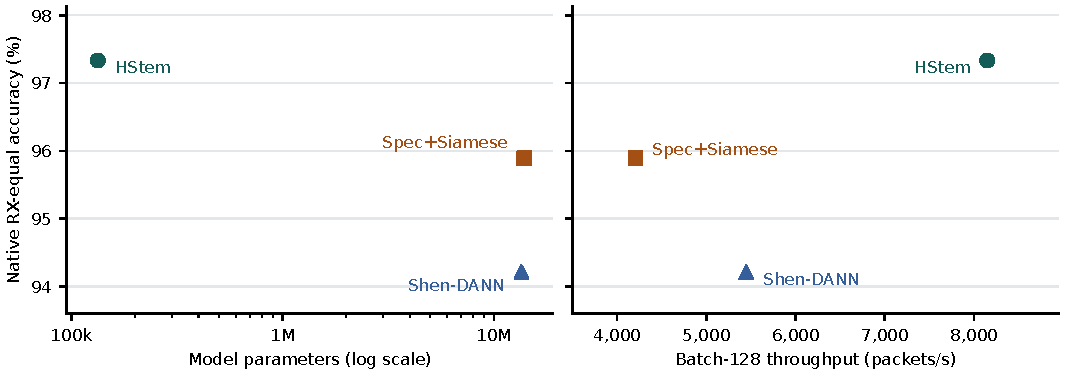
\includegraphics[width=.96\textwidth]{native_efficiency.pdf}
\caption{Native accuracy and efficiency for HStem, Spec+Siamese, and Shen-DANN in the common timing session. Left uses a logarithmic parameter axis. Right uses batch-128 throughput from the median synchronized batch latency.}
\label{fig:efficiency}
\end{figure*}

\begin{table*}[t]\centering
\caption{Native IQ-to-logits deployment costs on an RTX 4060 Laptop GPU. Accuracy is the receiver-equal mean across six fits. Costs use the first fold and seed, with identical GPU-resident IQ. B1/B128 batch times are p50/p95. Throughput is derived from B128 p50. MiB is the peak live PyTorch CUDA allocation at each batch size.}
\label{tab:costs}% Generated from the submission evidence ledger.
\begin{tabular}{lrrrrrr}
\toprule Method & Acc. (\%) & Parameters & B1 (ms) & B128 (ms) & B128 pkt/s & B1/B128 MiB\\
\midrule
HStem & 97.333 & 133,690 & 2.191 / 3.584 & 15.710 / 16.996 & 8,148 & 35.1 / 356.6\\
Spec+Siamese & 95.890 & 13,935,882 & 1.272 / 2.320 & 30.432 / 32.174 & 4,206 & 88.0 / 382.9\\
Shen-DANN & 94.208 & 13,509,263 & 1.195 / 2.207 & 23.498 / 24.795 & 5,447 & 85.2 / 328.5\\
\bottomrule
\end{tabular}

\end{table*}

Figure~\ref{fig:efficiency} shows the accuracy and efficiency trade-off. HStem uses 0.96\% of the parameters of Spec+Siamese and processes 8,451 packets/s at batch 128 in the shared GPU session, 1.96 times the Spec+Siamese rate. Median single-packet times are 1.865, 1.164, and 1.086\,ms for HStem, Spec+Siamese, and Shen-DANN, respectively.

The timing covers each method's complete native front-end and TX classifier under FP32 network inference with TF32 disabled. It starts with an extracted IQ window already on the device. Table~\ref{tab:costs} counts checkpoint parameters. The timed transmitter-only path uses 13,442,954 parameters for Shen-DANN. The supplement gives the full timing session and the earlier measurements.


\section{Tokenizer Ablations and Representation Analysis}
\subsection{Same-Support and Matched-Budget Comparisons}
In the matched GPU evaluation, HStem reaches 97.335\% versus 94.500\% for Long-Patch and 94.648\% for Patch-Lite. The 2.835\,pp HStem--Long-Patch gap has a conditional 95\% interval of \([2.253,3.530]\) pp, and all six paired fits favor HStem. Patch-Lite gives the closest parameter match and a 2.687\,pp gap. The change from Patch-Lite to the wider-support Long-Patch yields \(-0.148\)\,pp with a conditional interval of \([-0.765,0.312]\) pp. Together these comparisons support the staged tokenizer configuration at matched coordinate support and output geometry.

\begin{table*}[t]\centering
\caption{Matched LoRa tokenizer comparison. The three methods share the test packets and GPU inference session. Accuracy, F1, and worst RX are percentages.}
\label{tab:long}% Generated from the submission evidence ledger.
\begin{tabular}{lrrrrrr}
\toprule Tokenizer & Params & Support & BN & Acc. $\pm$ fit SD & F1 & Worst RX\\
\midrule
Patch-Lite & 134,266 & 266 & 2 & 94.648 $\pm$ 0.737 & 94.625 & 90.917\\
Long-Patch & 138,346 & 350 & 2 & 94.500 $\pm$ 1.831 & 94.423 & 88.333\\
HStem & 133,690 & 350 & 5 & 97.335 $\pm$ 0.552 & 97.326 & 93.667\\
\bottomrule
\end{tabular}

\end{table*}

\begin{figure*}[t]\centering
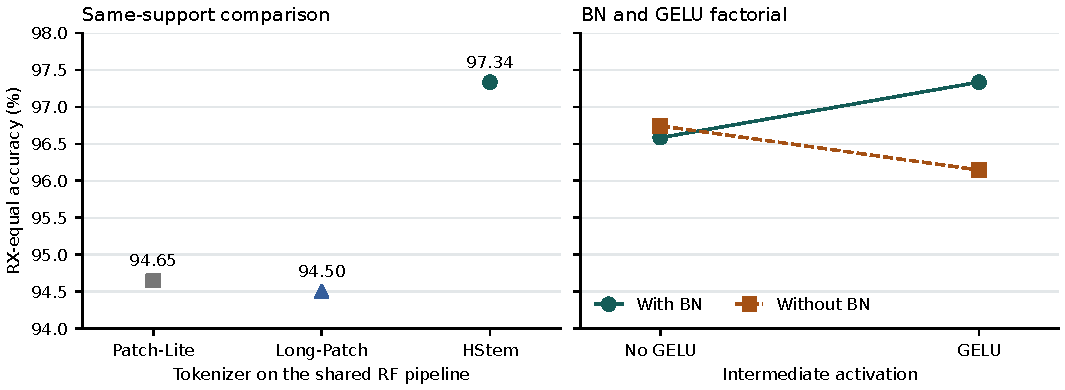
\includegraphics[width=.96\textwidth]{core_ablations.pdf}
\caption{Core tokenizer ablations. Left compares HStem with the support-matched Long-Patch and parameter-matched Patch-Lite controls. Right shows the change from adding intermediate GELU with and without intermediate BN. Both panels use RX-equal means.}
\label{fig:ablations}
\end{figure*}

\subsection{Parameterization and Normalization}
The full-rank round-trip parameterization improves Patch-Lite by \(0.878\)\,pp at unchanged support and folds back into a standard convolution at inference. The expanded-kernel configuration adds \(0.818\)\,pp. Removing intermediate BN reduces HStem accuracy by \(1.190\)\,pp, and restoring its affine parameters recovers \(0.272\)\,pp.

Adding intermediate GELU changes accuracy by \(+0.752\)\,pp with BN and \(-0.598\)\,pp without BN. The paired interaction is \(+1.350\)\,pp (conditional 95\% interval \([0.930,1.750]\) pp, Fig.~\ref{fig:ablations}). Removing intermediate BN and GELU leaves a staged affine tokenizer with a \(2.243\)\,pp higher observed mean than Long-Patch. The affine result is consistent with a role for factorized parameterization and its optimization. The supplement reports each contrast and its evaluation setting.


\subsection{Frozen Feature Geometry}
We examine 64-dimensional representations at the pooled tokenizer output, before MHA, and at the classifier input. The four configurations are evaluated on the same 2,000 source-validation packets per fold with frozen BN and per-packet L2 normalization. We summarize class separation and within-transmitter RX variation in this cohort.

For normalized $z_{tri}$, define global, TX, and TX-by-RX centroids $\mu,\mu_t,\mu_{tr}$. With $T=10,R=5,n=40$,
\begin{align}
 B_{\rm TX}&=T^{-1}\sum_t\|\mu_t-\mu\|^2,\\
 D_{\rm RX|TX}&=(TR)^{-1}\sum_{t,r}\|\mu_{tr}-\mu_t\|^2,\\
 W&=(TRn)^{-1}\sum_{t,r,i}\|z_{tri}-\mu_{tr}\|^2.
\end{align}
Total balanced scatter equals $B_{\rm TX}+D_{\rm RX|TX}+W$. We report
\begin{equation}
 J_c=\frac{B_{\rm TX}}{D_{\rm RX|TX}+10^{-12}},\quad
 J_w=\frac{B_{\rm TX}}{D_{\rm RX|TX}+W+10^{-12}}.
\end{equation}
At fixed group counts, $J_c$ is proportional to the ratio of between-TX centroid distance to same-TX cross-RX centroid distance.

\begin{table}[t]\centering
\caption{Feature geometry on source-validation packets. Each entry averages six per-fit statistics.}
\label{tab:source}% Generated from the submission evidence ledger.
\begin{tabular}{lrrrrr}
\toprule Arm & Source Acc. & $B_{\rm TX}$ & $D_{\rm RX|TX}$ & $J_c$ & $J_w$\\
\midrule
P0 & 95.917 & 0.785 & 0.0286 & 27.585 & 4.270\\
S1 & 96.625 & 0.778 & 0.0281 & 27.818 & 4.435\\
H1 & 97.467 & 0.805 & 0.0262 & 31.225 & 4.925\\
H0 & 98.175 & 0.817 & 0.0235 & 35.577 & 5.449\\
\bottomrule
\end{tabular}

\end{table}
\begin{figure*}[t]\centering
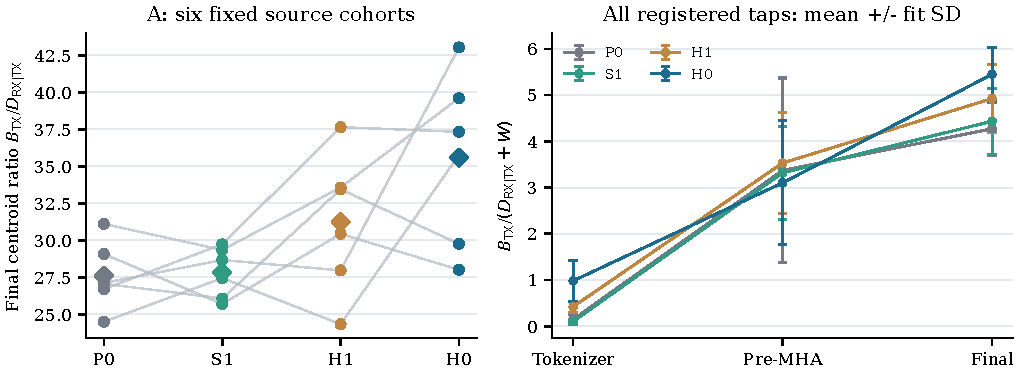
\includegraphics[width=.96\textwidth]{fig03_mechanism_A.pdf}
\caption{Final embedding separation across six fits and across layer taps. The final ordering emerges after the attention backend.}
\label{fig:geometry}
\end{figure*}

HStem's final mean \(J_w\) is \(5.449\), up \(27.6\%\) from Patch-Lite's \(4.270\), with a positive difference in all six source-validation pairs. Final \(J_c\) increases from \(27.585\) to \(35.577\), with five positive pairs. The intermediate ordering differs. HStem has larger conditional RX scatter at the tokenizer output (0.003004 versus 0.000185), and the pre-MHA \(J_c\) means are 33.983 for HStem and 41.241 for Patch-Lite. The final separation therefore reflects the representation formed by the staged tokenizer and attention together. Table~\ref{tab:source} and the supplement give the intermediate configurations and per-fit evidence.


\section{Cross-Waveform Evaluation}
The 8192-sample LoRa windows contain repeated chirps from chirp spread spectrum (CSS). As a stress test on another waveform, we use 256-sample WiSig ManyRx OFDM preambles, which expose short repeated training structures and timing boundaries \cite{hanna2022wisig,raychaudhuri2005orbit}. HStem and Long-Patch share a $32\times64$ interface and a 32-position support, with 82,426 and 82,364 parameters. Across two source-domain views, the comparison uses the same 22,968 packets and two matched seeds per view.

\begin{table}[t]\centering
\caption{Matched WiSig stress test. Positive values favor HStem. Differences and conditional 95\% RX intervals are in percentage points.}
\label{tab:wisig}% Generated from the submission evidence ledger.
\begin{tabular}{lrr}
\toprule Endpoint & Diff. & 95\% interval\\
\midrule
Natural-input accuracy & $+0.86$ & $[-0.22, +1.91]$\\
$\pm$10 kHz smaller loss & $+5.05$ & $[+2.88, +7.29]$\\
$\pm$9 samples smaller loss & $+3.51$ & $[+2.23, +4.77]$\\
\bottomrule
\end{tabular}

\end{table}

HStem reduces the accuracy loss by 5.05\,pp under $\pm$10 kHz offsets and by 3.51\,pp under $\pm$9-sample shifts compared with Long-Patch (Table~\ref{tab:wisig}). The shift comparison matches retained content and padding. The same table gives the natural-input difference and its conditional interval.

\section{Discussion and Conclusion}
Across matched LoRa fits, RF token construction changes accuracy even at the same nominal support and attention interface. Progressive tokenization yields a 2.835\,pp gain over Long-Patch. The parameterization and BN--GELU controls identify effects within the tokenizer, and the layerwise analysis locates the improved transmitter separation in the final embedding. Under the Native protocol HStem reaches 97.333\% accuracy and 93.683\% worst-RX accuracy. Relative to Spec+Siamese, it uses approximately one hundredth of the parameters and delivers 1.96 times the batch-128 throughput on the test GPU.

The LoRa result concerns aligned windows and ten enrolled TXs from receivers with documented development history. A four-sample circular shift reduces HStem source accuracy from 98.175\% to 21.858/17.775\% for negative/positive shifts, showing the importance of packet alignment. An independently acquired set with the same enrolled TXs is needed for prospective RX generalization, and security operating points such as unknown-emitter rejection require separate evaluation.

\appendices
\section{Reproduction Resources}
The \href{https://github.com/hanCChan/crossatten}{research repository} provides experiment definitions, evaluation code, figures, and aggregate results. The supplement describes the source-selected cohorts, numerical execution, training choices, and receiver-level analyses. The raw waveform archive, model weights, and packet predictions are maintained separately.

\IEEEtriggeratref{22}
\bibliographystyle{IEEEtran}
\bibliography{references}
\end{document}
